% !TEX root = ./main.tex
\chapter{Quantifying emissions spatial heterogeneity and mixing}
%\chapter{Quantifying emissions spatial heterogeneity, its contribution to atmospheric processes, and modeling parameterizations}

This chapter provides an overview of spatial heterogeneity (SH) and its relevance to quantifying the spatial variability of atmospheric emissions. We begin with a brief discussion of cross-disciplinary efforts to quantify SH. We then narrow our focus to quantifying the heterogeneity and mixing of reactive compounds in the atmosphere and characterize the gap in existing approaches that necessitate the development of a new, generally applicable SH metric that we will use in this thesis. The remainder of this chapter is dedicated to discussing our novel SH metric, the development of a Monte-Carlo based method for efficiently computing the metric over large domains, and its application to measuring the SH of idealized 2D patterns.  

\section{Existing approaches to quantifying spatial heterogeneity}\label{existing-sh-metrics}
SH is ubiquitous across the natural sciences ranging from ecology to atmospheric sciences. SH plays an important role in biological diversity, human land use and associated environmental feedbacks, and drives changes in atmospheric dynamics through spatially varying surface fluxes of heat, water vapor, and emissions. Despite its importance, quantifying SH is challenging in part because its definition can be highly dependent on the end use case. For instance, a metric used in geostatistics for measuring geographic variability in land use may not be particularly useful to an ecologist concerned with how spatially dependent a species population is on surrounding resources. Furthermore, mathematical assumptions central to the choice of metric such as scale similarity may not be applicable across use cases and thus limit the metrics' applicability. This has prompted the development of numerous metrics across disciplines that quantify SH. Here, we discuss various prominent SH metrics that range in applicability and complexity, and point to limitations in these approaches for use in quantifying emissions spatial heterogeneity. 

\subsection{Spatial autocorrelation and semivariograms}
Spatial correlation between measurements can be evaluated using correlograms and semivariograms. Correlograms are created by computing the correlation, measured via Pearson’s correlation coefficient, between two measurements separated by a given distance. Once the correlation across all distances and associated measurement pairs is computed, correlation is plotted against distance. A similar approach is employed for semivariograms, where the variance is plotted against distance between measurement pairs. \textcite{cooper_quantifying_1997} applied these techniques to determine the spatial correlation in streams between snail density and algal biomass, which serves as an important microhabitat. The authors showed how these metrics can be leveraged to quantify the spatial correlation and variability between measurements. While correlograms and semivariograms are useful for explaining the correlation and variance between spatially distributed measurements, they do not provide a one-point statistical measure of how spatially heterogeneous a region is, nor do they provide information on how variance for a quantity of interest is spatially arranged over a region.

\subsection{Fractal dimensions}
 A Fractal dimension, or fractional dimension, is a non-integer dimension \parencite{mandelbrot_how_1967, mandelbrot_fractal_1983}. Surfaces with greater complexity across spatial scales have higher fractal dimensions and vice versa. Fractal dimensions are scale invariant, meaning that they can be used to evaluate heterogeneity across surfaces of varying area. \textcite{loke_measuring_2022} discussed their use in ecology and pointed to numerous important limitations and considerations when utilizing fractal dimensions. The authors noted that in practice, measuring fractal dimensions is challenging due to the need to quantify the broad range of scales which may be limited by the resolution of measurement techniques. Additionally real-world objects and surfaces are not truly fractal because self-similarity breaks down at certain scales. 

\subsection{Lacunarity}
Surfaces with similar fractal dimensions can have dissimilar variations or texture (i.e., their variance can be arranged in different ways). This led \textcite{mandelbrot_fractal_1983} to introduce Lacunarity as a metric for quantifing the textural variation of surfaces with similar fractal dimension. Lacunarity is related to the distribution of scales of texture in a surface. Surfaces with a broader range of texture, including large and small gaps and variations, will tend to have high lacunarity. For more homogeneous objects, the distribution of texture scales will be narrower and will result in a lower lacunarity value. \textcite{dong_lacunarity_2000} provided an overview of lacunarity and its use in geography and geographic information science (GIS) applications. They noted that lacunarity is often quantified using a gliding box algorithm, for which the researcher must choose the gliding box size. Importantly, changes to the gliding box size do not ensure linear scaling of the difference between lacunarity of multiple patches, meaning that, for instance, a patch may have higher lacunarity compared to other patches at small gliding box sizes but may have lower lacunarity than other patches at larger gliding box size. While this may be a useful attribute of lacunarity if one wishes to evaluate the scale dependence of spatial variability and the scales at which patches appear spatially similar or dissimilar as is the use case as outlined by \textcite{dong_lacunarity_2000}, gliding box size introduces an additional parameter one must choose when quantifying spatial heterogeneity and could complicate intercomparison of lacunarity measurements.

\subsection{Information entropy based metrics}
In landscape ecology, information entropy based metrics such as Shannon’s evenness index are used to quantify the patchiness of topography that is divided among numerous land uses classes. \textcite{plexida_selecting_2014} evaluated a number of metrics, including Shannon’s evenness index, for measuring the topological variability and land use of central Greece. For its use in landscape ecology, Shannon’s evenness quantifies how evenly distributed the various land use types in a region are. It is defined as Shannon’s diversity index over $N$ populations (i.e., the Shannon entropy) divided by the maximum diversity index. Shannon's evenness index is useful if evaluating a region with numerous patches that are divided into different categories; however, its use is less apparent for quantifying the spatial heterogeneity of a single scalar field.

\subsection{Nearest neighbor statistics for point-based heterogeneity}
\textcite{shu_quantifying_2019} discussed nearest neighbor distance statistics for use in GIS settings to quantify the spatial heterogeneity of points and apply various metrics to example cases including the spatial distribution of crime events in a city, regional seismic activity in Yutian China, and taxi routes in Beijing China.  Examples ranged from 2D to 4D, illustrating the multidimensional applicability of nearest-neighbor metrics. The authors presented a goodness-of-fit metric based on the distribution of nearest neighbor distances called the level of heterogeneity. A normalized version of the metric was proposed to resolve issues that arise when comparing datasets with differing magnitudes due to differences in scale or intensity. The authors noted that while the proposed metric is suitable for capturing point-based spatial heterogeneity, it is quite computationally expensive. It was recommended that alternative nearest-neighbor metrics evaluated alongside the proposed metric should be preferred for computationally intensive datasets. 

\subsection{Multiscale norms}
Sobolev norms have been used to quantify the mixing and transport of passive scalars in fluids \parencite{thiffeault_using_2012}. Sobolev norms act as a weighted sum of the Fourier coefficients resulting from the Fourier transform of a scalar field (i.e, the passive scalar suspended in either a fluid or the atmosphere). The multiscale nature of Sobolev norms refers to the selection of Sobolev space $H^q$ over which the norm is defined. \textcite{thiffeault_using_2012} showed that the choice of Sobolev norm for $q<0$ is valuable for flow mixing applications as the magnitude of the norm decays alongside the mixing of the medium.

\section{Metrics for quantifying the mixing of reactive compounds}\label{metrics-reactive-mixing}
Atmospheric constituents that undergo chemical reactions including gas phase and aerosol species are subject to both spatial and temporal constraints that determine the rate at which reactions will proceed. For instance, species must be spatially collocated for reactions to occur, and they must remain in close proximity over the timescale that a given reaction will proceed. This gives rise to two important metrics: (1) segregation intensity, which quantifies the spatial proximity of reactive species and (2) the Damköhler number, which characterizes the dominant timescales governing the reactivity of species.

\subsection{Segregation intensity}
The segregation intensity, first theorized by \textcite{danckwerts_definition_1952} for use in combustion processes, is a measure of how spatially segregated or mixed two reactive species are that follow a typical second-order reaction of the form

\begin{equation}
\ce{A + B -> C}.
\end{equation}
Using Reynolds decomposition to express each species concentration as the sum of a spatial average and local deviation, $[A] = \overline{[A]} + [A]'$, $[B] = \overline{[B]} + [B]'$, such that the  chemical reaction proceeds as 
\begin{equation}
\frac{d[A]}{dt} = \frac{d[B]}{dt} = -k\left(\overline{[A]}\cdot\overline{[B]} + \overline{[A'][B']} \right).
\end{equation}
The segregation intensity is then 
\begin{equation}
I_s = \frac{\overline{[A'][B']}}{\overline{[A]}\cdot\overline{[B]}},
\end{equation}
such that the chemical reaction can be expressed as 
\begin{equation}
\frac{d[A]}{dt} = \frac{d[B]}{dt} = -k\left(\overline{[A]}\cdot\overline{[B]}\right)\left(1 + I_s \right).
\end{equation}
Thus, $I_s$ can be thought of as imposing an effective reaction rate $k^{\text{eff}} = k(1+I_s)$. When $I_s = -1$, species $A$ and $B$ are fully spatially separated, such that no reaction occurs. As $I_s$ approaches zero, the two species become fully mixed and the effective reaction rate matches the ideal rate of reaction. $I_s$ can also be positive, corresponding to positive covariance between species which effectively increases the rate of reaction.

\subsection{Damköhler number}
The Damköhler number \parencite{damköhler_effect_1947} relates the turbulence and chemical reaction timescales via the ratio
\begin{equation}
D_a = \frac{\tau_{\text{turb}}}{\tau_{\text{chem}}}.
\end{equation}
%where $\tau_{\text{turb}} = $ and $\tau_{\text{chem}} = $
The definition of turbulent and chemical timescales varies by application. For the convective boundary layer, \textcite{vinuesa_fluxes_2003} adopted the following expression for the Damköhler number,
\begin{equation}
D_a = \frac{z_i}{w_*}k[B],
\end{equation}
where $w_*$ is the velocity scale in the convective boundary layer and is defined as $\left[(g/\Theta_v)\overline{w\theta}_0 z_i\right]^{1/3}$, and where $g$ is gravitational acceleration, $\Theta_v$ is virtual potential temperature, $\overline{w\theta}_0$ is vertical heat flux, and $z_i$ is the boundary layer height.

\begin{figure}[h]
	\centering
	\includegraphics[width=\textwidth]{figures/chapter2/damkohler_number_figure.pdf}
	\caption{Dependence of the Damköhler number on turbulent and reactive timescales. Figure adapted from \textcite{kotamarthi_and_2017}}
	\label{fig:damkohler}
\end{figure}

Figure \ref{fig:damkohler} displays the three primary regimes for the Damköhler number that determine the abundance of precursor concentrations $[A]$ and $[B]$. When the turbulent and chemical timescales are balanced, $D_a = 1$. If the chemical reaction timescale is shorter than the turbulence timescale, $D_a >1$ and the concentration of the precursors will be determined by the rate at which turbulence mixes the reactive compounds (fast-chemistry regime). Conversely, if the chemical reaction timescale is slower than the turbulent timescale, $D_a<1$ such that the concentration of precursors is determined by the rate of chemical reaction (slow-chemistry regime). Thus, the Damköhler number indicates the relative importance of turbulence in chemical reactions -- in the fast chemistry regime with  reactions with $D_a > 1$, turbulent scales responsible for mixing the reactive compounds should be fully resolved. Examples of relevant gas-phase reactions in convective boundary layer that correspond to the fast-chemistry regime include oxidation of volatile organic compounds such as isoprene by OH to produce semi-volatile organic compounds that partition into the aerosol phase to form secondary organic aerosol. Additional fast reactions include the oxidation of SO$_2$ by OH, resulting in H$_2$SO$_4$ which posses an extremely low volatility and rapidly condenses into the aerosol phase where it forms sulfate (SO$_4^{2-}$). 

\section{A novel approach to quantifying spatial heterogeneity}
Existing approaches to quantifying spatial heterogeneity discussed in Section \ref{existing-sh-metrics} and metrics for mixing of reactive compounds in Section \ref{metrics-reactive-mixing} provide valuable information on the state of a heterogeneously distributed field, however each metric varies in terms of range of applicability, interpretability, and ease of implementation. 

For instance, spatial autocorrelation and semivariograms are relatively easy to interpret and are computationally efficient to measure, but they are primarily useful for capturing the correlation and variability at a single point rather than over an entire region. Alternatively, the nearest neighbor metric proposed by \textcite{shu_quantifying_2019} is useful across a broad range of applications as illustrated by the authors, however, their approach is computationally expensive and is not readily interpretable to the same manner as other spatial heterogeneity metrics. Metrics for mixing provide useful information on how spatially colocated reactive compounds are and the relevant timescales that determine the abundance of precursors, however they do not provide information on how the variance in the spatial distribution of each compound is arranged. 

Thus, there exists the need for a novel spatial heterogeneity metric for use in atmospheric science applications including quantifying emissions spatial heterogeneity and subsequent atmospheric field heterogeneity once compounds are emitted into the planetary boundary layer. \textcite{mohebalhojeh_2024} have developed a new approach to measuring spatial heterogeneity with key benefits being that their approach is broadly applicable, straightforward to interpret, and computationally efficient to measure using a Monte Carlo approach discussed in Section \ref{sh-metric-calculation}.

\subsection{Metric definition}
The spatial heterogeneity metric, subsequently $SH$, quantifies the level of heterogeneity for single scalar quantity over a 2-dimensional surface. In this thesis, the scalar of interest is either gas phase or aerosol species and the 2-dimensional surface is either the ground level in the case of emissions or a horizontal plane through the computational domain to quantify atmospheric field heterogeneity within the planetary boundary layer.

$SH$ is calculated by summing up the absolute difference between the mean of a scalar quantity over a rectangular subset of the domain and the domain averaged value for all possible subsets. Over a discrete 2-dimensional grid with $N$ cells along the x-axis and $M$ along the y-axis, there exist \\$P=(N(N-1)+1)(M(M-1)+1)$ total possible rectangular subsets. For a scalar field $f$ defined over some domain $S$, $SH$ is computed as

\begin{equation}
SH(f, S) = \frac{1}{P}\sum_{\tilde{S}\in \mathbb{R}}|\overline{f}(S) - \overline{f}(\tilde{S})|.
\end{equation}

\begin{figure}[!t]
	\centering
	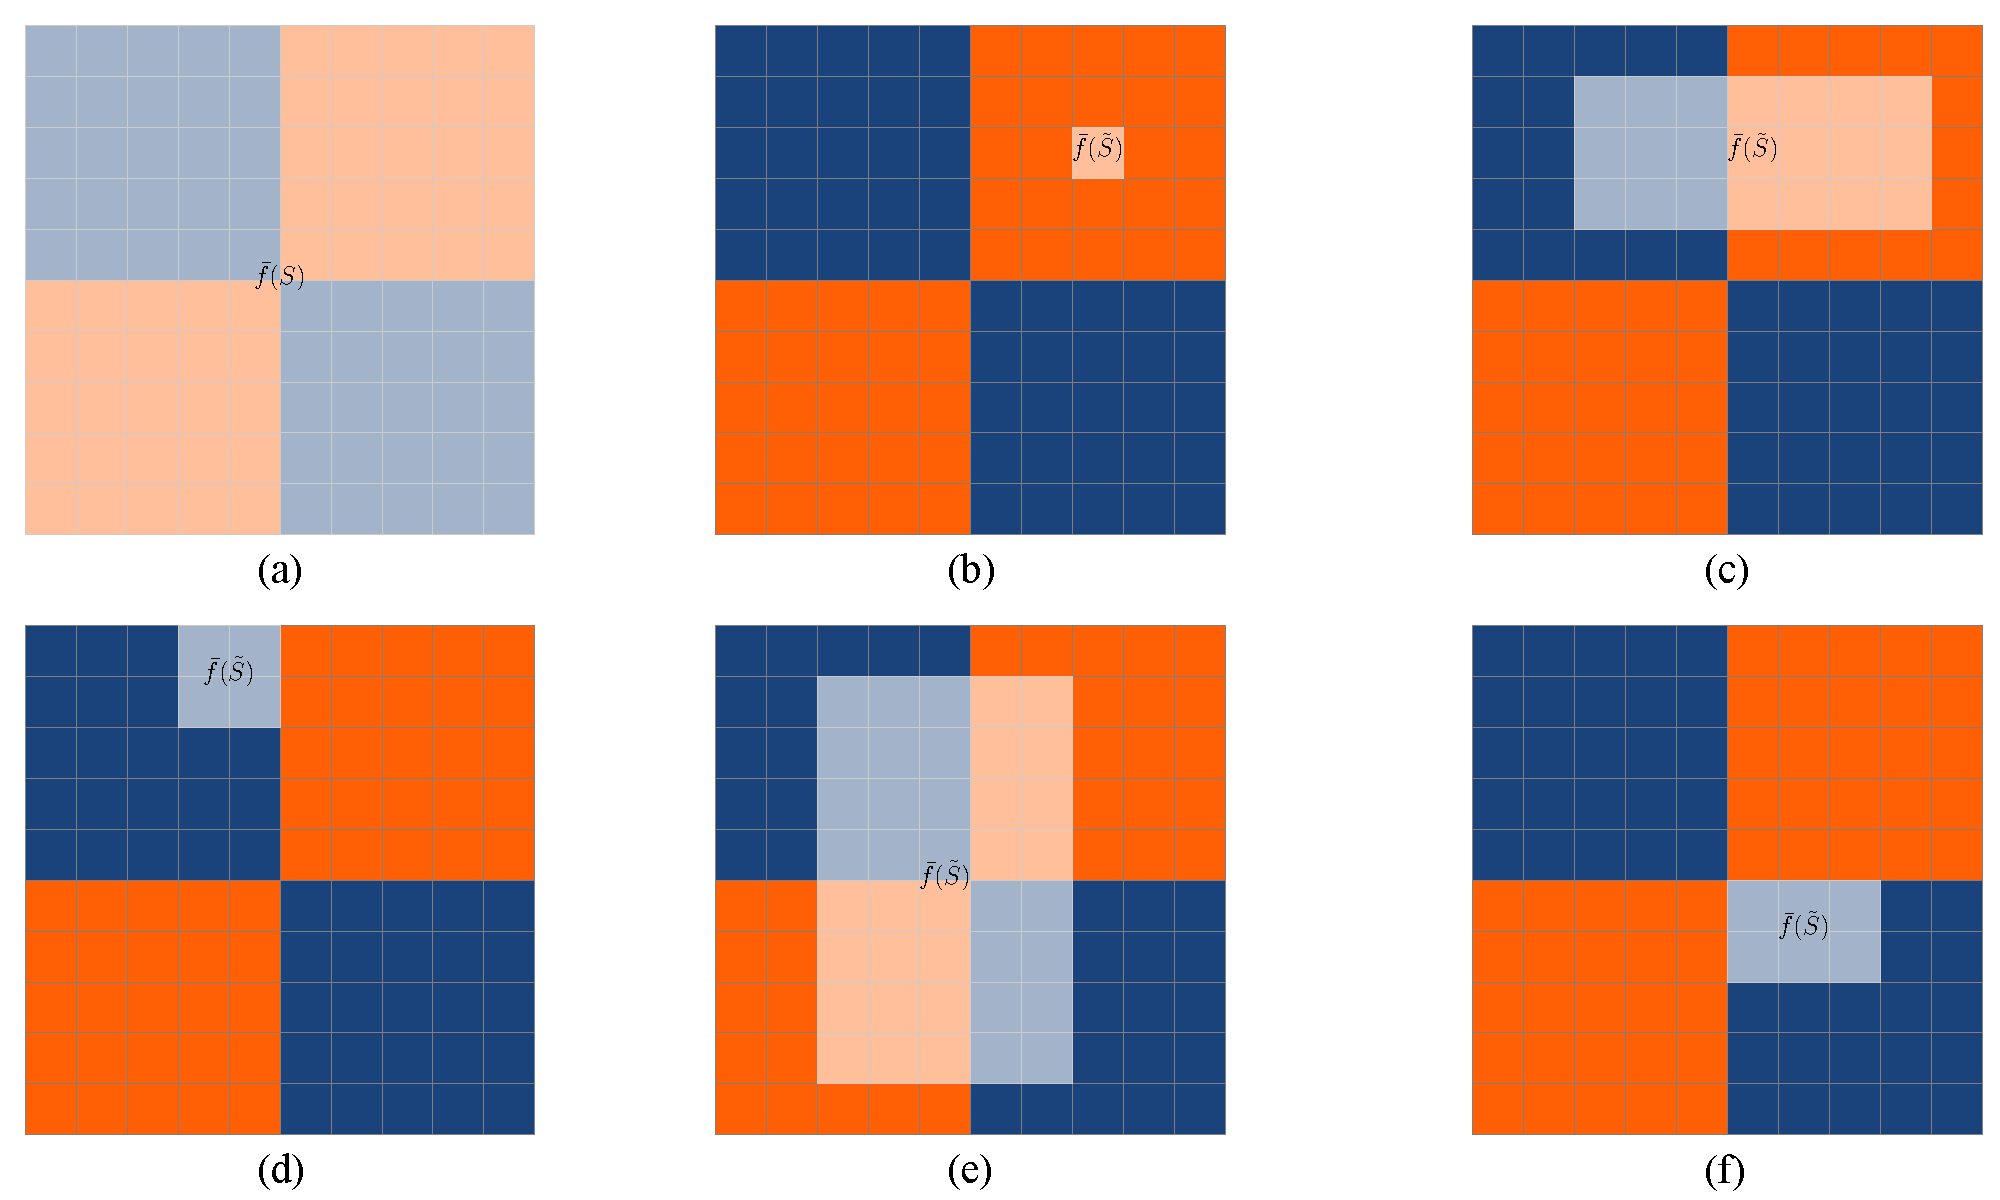
\includegraphics[width=\textwidth]{figures/chapter2/SH-subarray-examples.pdf}
	\caption{Example subsets for $SH$ calculation. (a) Full domain mean. (b-f) Examples of rectangular subsets (highlighted regions) over which the subset mean is computed.}
	\label{fig:sh-subarrays}
\end{figure}

Because the range of gas phase and aerosol emissions varies across orders of magnitude, it is useful to instead utilize a normalized version of the spatial heterogeneity metric,

\begin{equation}
SH(f, S) = \frac{1}{\overline{f}(S)\left[\frac{3}{2}(N\times M)(N-1)(M-1) + N(N-1) + M(M-1)\right]}\sum_{\tilde{S}\in \mathbb{R}}|\overline{f}(S) - \overline{f}(\tilde{S})|.
\end{equation}

The normalized spatial heterogeneity metric possesses values in the range $[0, 1]$. The metric is defined for two-dimensional rectangular surfaces with periodic boundaries. \textcite{mohebalhojeh_2024} show that the metric is translationally invariant when the scalar field $f$ is translated over the domain $S$. Furthermore, it is presented in theorem and proof that the maximum spatial heterogeneity over a discrete domain occurs when the value of the scalar field is zero everywhere except at a single point at which it takes the value $MN\times\overline{f}$. Referred to as the ``spatial heterogeneity maximum theorem", it is of particular importance to this thesis, as we shall present modeling runs corresponding to a variety of emissions spatial heterogeneity scenarios including the maximally heterogeneous scenario. 

A visualization of the total domain mean $\overline{f}(S)$ and domain subset means $\overline{f}(\tilde{S})$ are shown in Figure \ref{fig:sh-subarrays}. The checkerboard pattern represents an idealized emission pattern, where orange-filled cells correspond to regions of uniform emissions and dark blue regions correspond to zero emissions. $\overline{f}(S)$ is shown in subfigure (a), while five examples of rectangular subsets are displayed in subfigures (b-f).


\subsection{Computational methods for computing the spatial heterogeneity metric}\label{sh-metric-calculation}
To calculate $SH$ over a computational domain, an array comprising the scalar quantity of interest with dimension equal to the size of the domain ($N$ by $M$) is passed to a Fortran subroutine. Here, we discuss two approaches to calculating $SH$: a computationally expensive naive looping algorithm and a significantly more efficient Monte Carlo based method.

\begin{figure}[!t]
	\centering
	\includegraphics[width=\textwidth]{figures/chapter2/NSH-performance.pdf}
	\caption{CPU time for the naive looping $SH$ Fortran subroutine. The x-axis indicates the total number of domain grid cells (elements) in the array passed to the subroutine. A power law regression is plotted as the red dashed line.}
	\label{fig:nsh-performance}
\end{figure}

The naive subroutine loops over all possible rectangular subdomains which can be quite computationally expensive, especially for domains with a large number of grid cells (e.g., 100$\times$100 grid cells laterally as used for domain mesh size in this thesis). Figure \ref{fig:nsh-performance} shows the computational scaling for a Fortran subroutine using this naive looping algorithm. A power law regression (red dashed lined) is fit to the CPU time vs. the total number of domain grid cells. The naive looping algorithm scales as $O(n^3)$ for $n$ the number of grid cels. For domain sizes used in this thesis ($N=M=100$), this results in a single calculation taking in excess of 2~minutes.

\begin{figure}[!t]
	\centering
	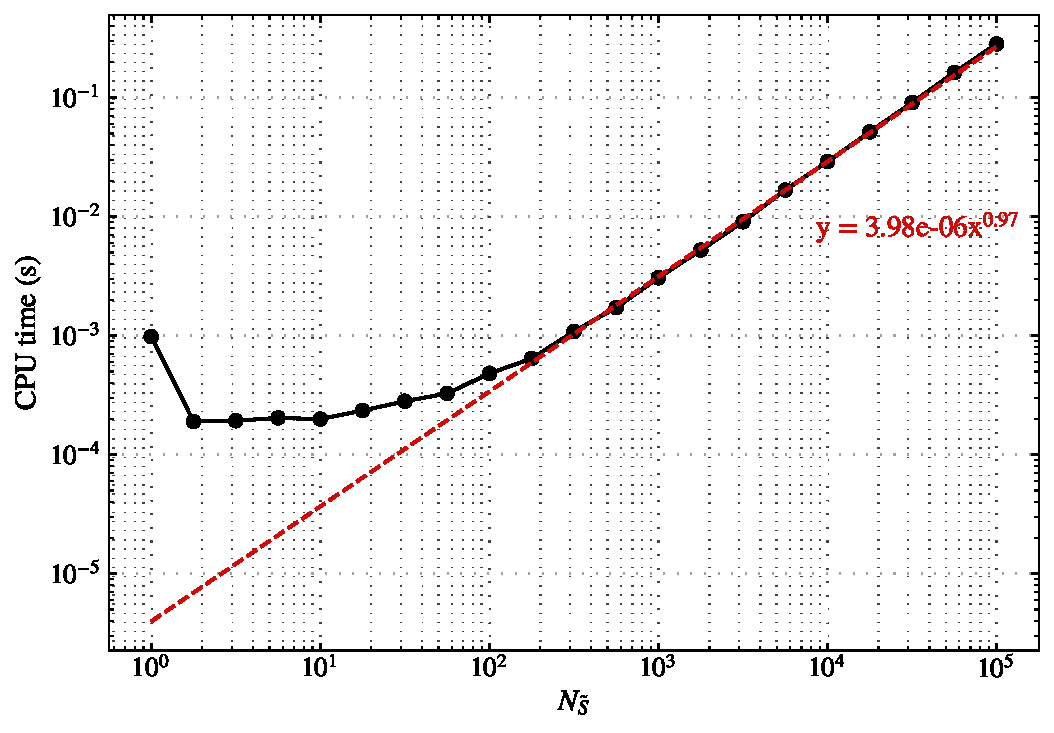
\includegraphics[width=\textwidth]{figures/chapter2/mcNSH-performance.pdf}
	\caption{CPU time for the Monte Carlo $SH$ Fortran subroutine. The x-axis indicates the number of domain subsets that are randomly selected to determine the $SH$ estimate. A power law regression is plotted as the red dashed line.}
	\label{fig:mcsh-performance}
\end{figure}

Instead of looping over every possible subdomain, we may use the fact that the probability of selecting any given subdomain is the same (i.e., the sampling probability is uniform across the entire domain) in order to construct a Monte Carlo sampling based approach for calculating $SH$. We then pass the array with domain scalar values alongside a parameter for the number of subsets to sample ($N_{\tilde{S}}$) to our Monte Carlo-based Fortran subroutine. Figure \ref{fig:mcsh-performance} shows the CPU time for corresponding number of randomly selected domain subsets, ranging from 1 to 100,000 for a domain with dimensions $N=M=100$ and $P=(100(100-1)+1)(100(100-1)+1) = 98,029,801$ total subsets. For a low number of randomly selected subsets (number of subdomains $\lesssim 100$), the algorithm scales quite weakly, suggesting that computational overhead limits speedup in this region over the naive algorithm. As the number of subdomains increases above 100, the algorithm scales as $O(N_{\tilde{S}})$ as indicated by the power law regression.

\begin{figure}[!t]
	\centering
	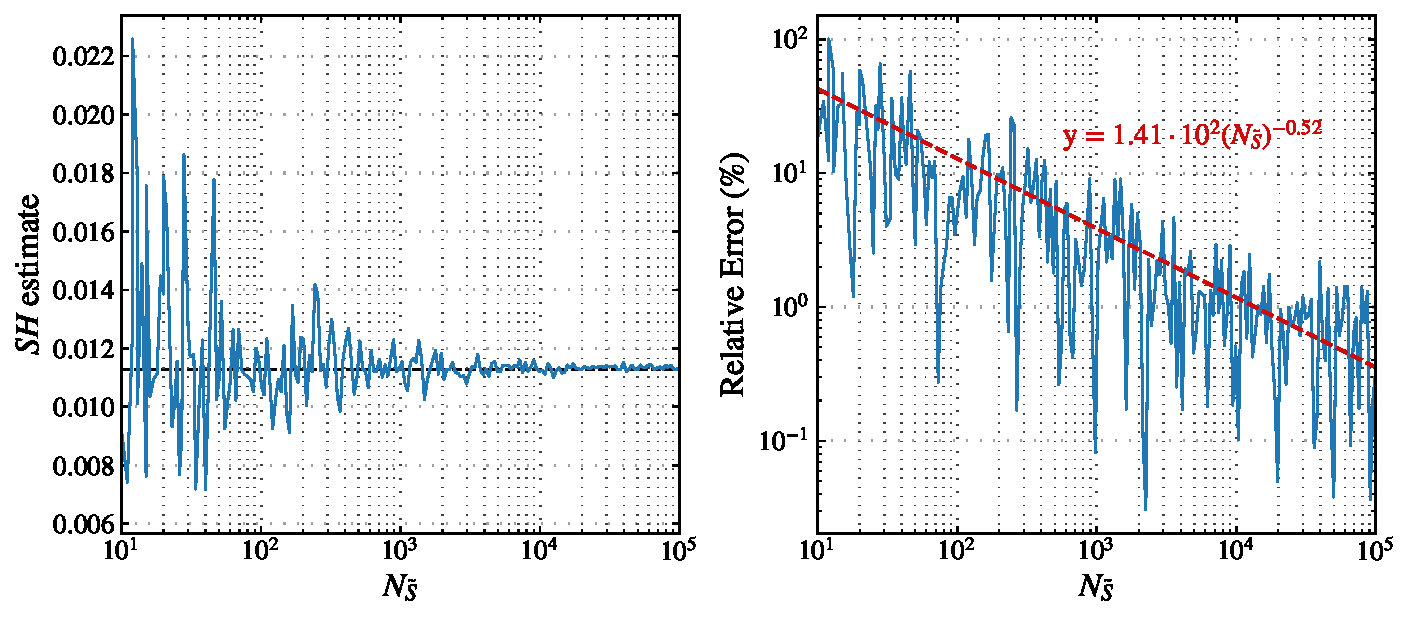
\includegraphics[width=\textwidth]{figures/chapter2/mcNSH-accuracy-v2.pdf}
	\caption{$SH$ estimate in blue for the Monte Carlo sampling subroutine vs. the number of randomly selected domain subsets (left). The true value of $SH$ computed via the naive algorithm is shown as the black line. Relative error is shown between $SH$ estimates and the true value of $SH$ (right) }
	\label{fig:mcsh-accuracy}
\end{figure}

We validate the accuracy of the Monte Carlo sampling subroutine against the naive looping approach in Figure \ref{fig:mcsh-accuracy}. First, the precise value of $SH$ was computed via the naive algorithm for a scalar field of random noise with dimensions $N=M=100$. We then vary the number of randomly selected subsets $N_{\tilde{S}}$ used to compute the estimate of $SH$ in the Monte-Carlo subroutine. The left panel in Figure \ref{fig:mcsh-accuracy} shows how the $SH$ estimate converges on the precise value of $SH$ (shown as a horizontal black dashed line). The right panel displays the relative error between $SH$ estimates and the precise value (note the logarithmic scaling). Relative error decreases as $\propto 1/\sqrt{N_{\tilde{S}}}$ as indicated by the power law regression in red. This behavior is to be expected, because as the number of samples (i.e., $N_{\tilde{S}}$) increases, the error should decrease like the standard error-- $SE = \sigma/\sqrt{n}$ for $\sigma$ the standard deviation of a sampling distribution and $n$ the number of samples.

Given the performance of the Monte Carlo sampling subroutine over the naive looping approach and its ability to reach a high level of accuracy with minimal error when sampling a sufficient number of domain subsets, we utilize the Monte Carlo method for subsequent $SH$ calculations. For such calculations, we choose the number of randomly selected domain subsets to be 10,000 as this results in relative error $\sim 1\%$ for the domain size $N=M=100$ used in this thesis. Referring back to Figures \ref{fig:nsh-performance} and \ref{fig:mcsh-performance} for naive algorithm performance and Monte Carlo sampling performance, respectively, we find that for a domain size with $N=M=100$, CPU time is in excess of two minutes for the naive looping approach and of order $\sim0.1$ \si{s} for the Monte Carlo subroutine. This corresponds to a speedup in excess of 1000.

\subsection{Example calculations for emission patterns}

\begin{figure}[!t]
	\centering
	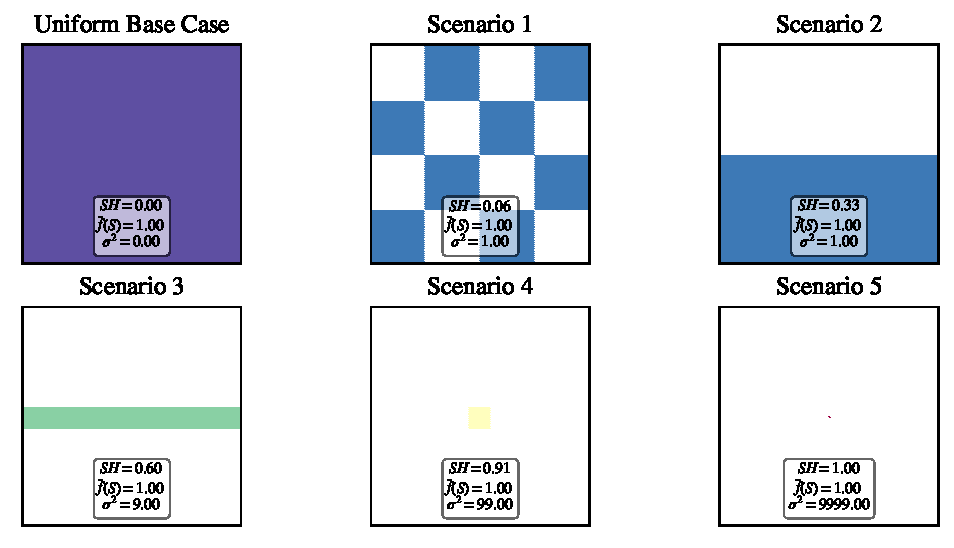
\includegraphics[width=\textwidth]{figures/chapter2/SH-scenarios-all.pdf}
	\caption{Example emission patterns arranged from least heterogeneous (``Uniform Base Case") to most heterogeneous (``Scenario 5").  For each pattern, the spatial heterogeneity $SH$ is listed alongside the domain mean ($\overline{f}(S)$) and variance ($\sigma^2$). The color of each scenario indicates the emission scaling relative to the uniform base case with red being the highest scaling.)}
	\label{fig:emission-patterns}
\end{figure}

We calculate the spatial heterogeneity for 6 emission scenarios shown in Figure \ref{fig:emission-patterns}. Emission patterns are ordered from low to high $SH$, ranging from uniform emissions across the domain (``Uniform Base Case") to highly heterogeneous localized emissions. Note that the total mass of emissions per unit time is the same across all scenarios. The emissions scaling rate is adjusted based on the area each pattern occupies relative to the base case and is indicated by the color of each emission region (dark blue corresponds to scaling closer to unity while red indicates the greatest magnitude of scaling). 

For each scenario, the domain mean, $\overline{f}(S)$, and variance, $\sigma^2$, are shown in addition to $SH$. Note that the variance of the checkerboard scenarios 1 and 2 are all equal to 1.0 while the $SH$ increases across these scenarios. This highlights an important attribute of the spatial heterogeneity metric--the $SH$ metric provides information not only on how variable an emission pattern is across the domain, but also is sensitive to how the variance is arranged. This marks an advantage of the $SH$ metric over previously discussed metrics, including semivariograms, fractal dimensions, and information entropy statistical measures that are insensitive to changes in the distribution of variance over the scalar field of interest.
